% XCircuit output "outputprot.tex" for LaTeX input from outputprot.eps
\def\putbox#1#2#3#4{\makebox[0in][l]{\makebox[#1][l]{}\raisebox{\baselineskip}[0in][0in]{\raisebox{#2}[0in][0in]{\scalebox{#3}{#4}}}}}
\def\rightbox#1{\makebox[0in][r]{#1}}
\def\centbox#1{\makebox[0in]{#1}}
\def\topbox#1{\raisebox{-0.60\baselineskip}[0in][0in]{#1}}
\def\midbox#1{\raisebox{-0.20\baselineskip}[0in][0in]{#1}}
   \scalebox{0.7}{
   \normalsize
   \parbox{3.98437in}{
   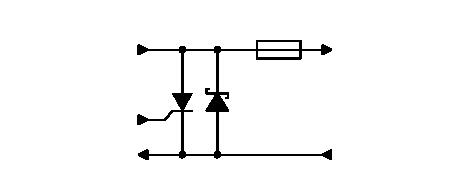
\includegraphics[scale=1.42857]{outputprot}\\
   % translate x=690 y=240 scale 0.26
   \putbox{1.08in}{1.40in}{1.20}{\rightbox{\midbox{From}}}%
   \putbox{1.08in}{1.23in}{1.20}{\rightbox{\midbox{Output}}}%
   \putbox{1.08in}{1.07in}{1.20}{\rightbox{\midbox{Amplifier}}}%
   \putbox{1.08in}{0.65in}{1.20}{\rightbox{\midbox{Thyristor}}}%
   \putbox{1.08in}{0.48in}{1.20}{\rightbox{\midbox{Trip}}}%
   \putbox{1.08in}{0.32in}{1.20}{\rightbox{\midbox{To Current}}}%
   \putbox{1.08in}{0.15in}{1.20}{\rightbox{\midbox{Sense}}}%
   \putbox{3.08in}{1.23in}{1.20}{\midbox{Output$+$}}%
   \putbox{3.08in}{0.23in}{1.20}{\midbox{Output$-$}}%
   \putbox{1.41in}{0.98in}{1.20}{\centbox{\midbox{\rd{Q2}}}}%
   \putbox{2.08in}{0.98in}{1.20}{\centbox{\midbox{\rd{D1}}}}%
   \putbox{2.50in}{1.48in}{1.20}{\centbox{\midbox{\rd{F1}}}}%
   } % close 'parbox'
   } % close 'scalebox'
   \vspace{-\baselineskip} % this is not necessary, but looks better
